\chapter{Krabička}
%Základna Jako poslední část jsem potřebovala krabičku – nějakou základnu, která by sjednotila jednotlivé komponenty do jednoho kompletního celku. 
Jako poslední už mi zbývalo jen udělat krabičku, nebo také základnu, do které bych mohla schovat Elektrický obvod, a na vršek umístit růži.
Rozměry krabičky byly designované podle nejrozměrnější komponenty v elektrickém obvodu, se jednalo o držák s bateriemi, jehož rozměry jsou 75~mm x 42~mm x a na výšku 20~mm. Druhou největší komponenta byla deska \textit{ESP32-DevKitC} s rozměry: 55m~m x 30~mm s~výškou 10~mm.
Podle výše zmíněných dvou nevětších komponent byly stanoveny přibližné vnitřní rozměry základny: 82~mm x 82~mm x 45~mm, které zaručovaly, že se do základny vejde jak \textit{ESP32-DevKitC} tak baterky, zůstane nějaká rezerva na kabely a další komponenty a základna nebude o moc větší než růže.  
Aby byla ověřena správnost rozměrů, byl podle nich vytvořen první prototyp.
%abych ověřila správnost rozměrů, rozhodla jsem se podle nich vytvořit první prototyp.
%82 mm x 82 mm x 45 mm,



\section{První prototyp}
První prototyp byl vyroben ručně ze 4~mm široké překližky. Podle toho se poté přibližně odvodily vnější rozměry základny. U tohoto prototypu to přibližně bylo: 90 x 90 x 50~mm. Tato práce nebyla profesionální, proto se výsledné rozměry základny nepatrně lišily (+/-2~mm).
%jsem vyrobila ručně

Pro výrobu prototypu bylo z překližky vyřezáno šest dílů: Vrchní a spodní díl 90~mm x 90~mm, a 4 boční stěny o rozměrech 45 x 90~mm a 45 x 82~mm. Do vrchního dílu byl vyřezán kruhový otvor o průměru 28~mm, pro umístění odlité růže a do jednoho bočního dílu vyvrtala vrtačkou otvor pro menší přepínací tlačítko. Do rohů byly přilepeny lepidlem \textit{Herkules} špalíčky 10~x~10~mm, které držely všechny desky základny u sebe a později sloužily pro držení vrchního dílu a růží pomocí šroubků. Takže se vrchní díl s růží mohl kdykoliv sundat a bylo možné manipulovat s elektrotechnikou uvnitř.

%todo jak je to s přívlastky? 
%Dva čtverce o šířce přibližně 90 mm
%2 obdélníky o výšce 45 mm a délce 90
%2 obdélníky o výšce 45 mm a délce 82
\begin{figure}[htbp]
	\centering
	\begin{minipage}[b]{0.5\textwidth}
		\centering
		\includegraphics[width=0.8\textwidth]{img/06 zakl/Ama základna.jpg}
		\caption{První prototyp}
		%		\label{fig:gear-sketch1}
	\end{minipage}
	\qquad
	\begin{minipage}[b]{0.4\textwidth}
		\centering
		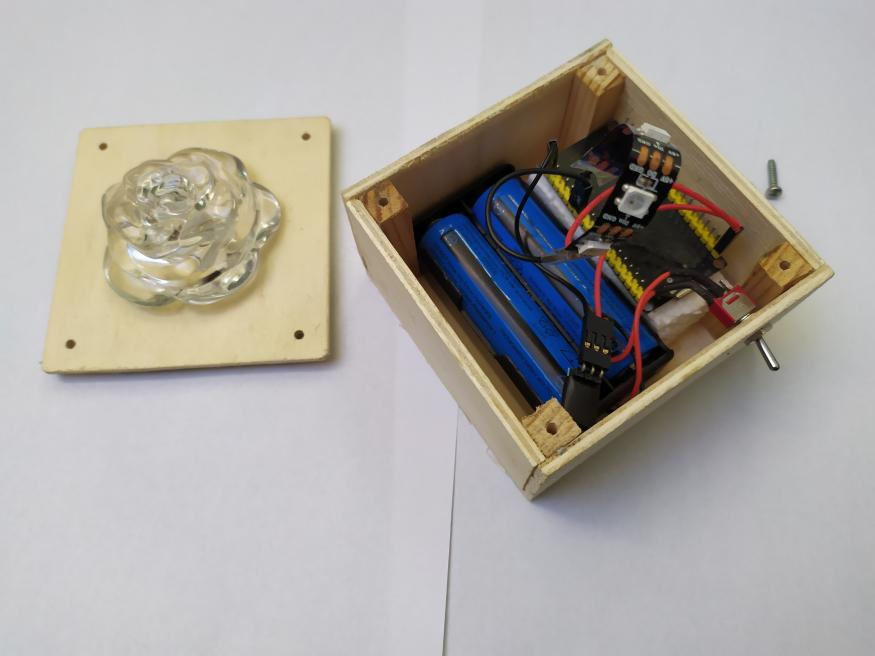
\includegraphics[width=1\textwidth]{img/06 zakl/1. prototyp s ele.jpg}
		\caption{Kompletní  prototyp}
		%		\label{fig:gear-sketch2}
	\end{minipage}
\end{figure}

Po sestavení krabičky byl pro kontrolu do krabičky vložen náš elektrický obvod.
Jelikož pokus s prvním prototypem proběhl úspěšně, začala jsem pracovat na dokonalejším druhém prototypu.


\section{Druhý prototyp základny }
Druhý prototyp základny byl také vyroben ze dřeva, tentokrát ale byly jednotlivé stěny krabice vypáleny na laseru. Díky čemuž prototyp působil profesionálněji. Při této výrobě byla použita překližka široká 3~mm. Jednotlivé díly krabičky byly navrženy programu MakerCaser, který po zadání vnitřních rozměrů a rozměrů překližky, vygeneroval výkres hotové krabičky i s hotovými okrajovými zámky, aby se do rohů prototypu tentokrát nemuseli lepit špalíčky. 

\textit{Lightburn}\cite{lightburn}.

\subsection{Práce s Lightburnem}
\textit{Lightburn} je placený editační software, který škola používá pro práci s laserovými řezačkami. 
Snačilo do tohoto programu poze nahrát uložený soubor ze stránky \textit{MakerCaser}\cite{makercase}, přidat otvor ve vrchním dílu a logo školy. Poté stačilo upravený soubor nahrát ve formátu .svg do školní Laserové tiskárny a krabičku vypálit. Výsledek působil reprezentativně, takže se nakonec na laseru vypálily i krabičky pro zbývající výrobky. 
 %Jinak zbytek ostatní  zůstal beze změny.


%todo *Obrázek*

\begin{figure}[htbp]
	\centering
	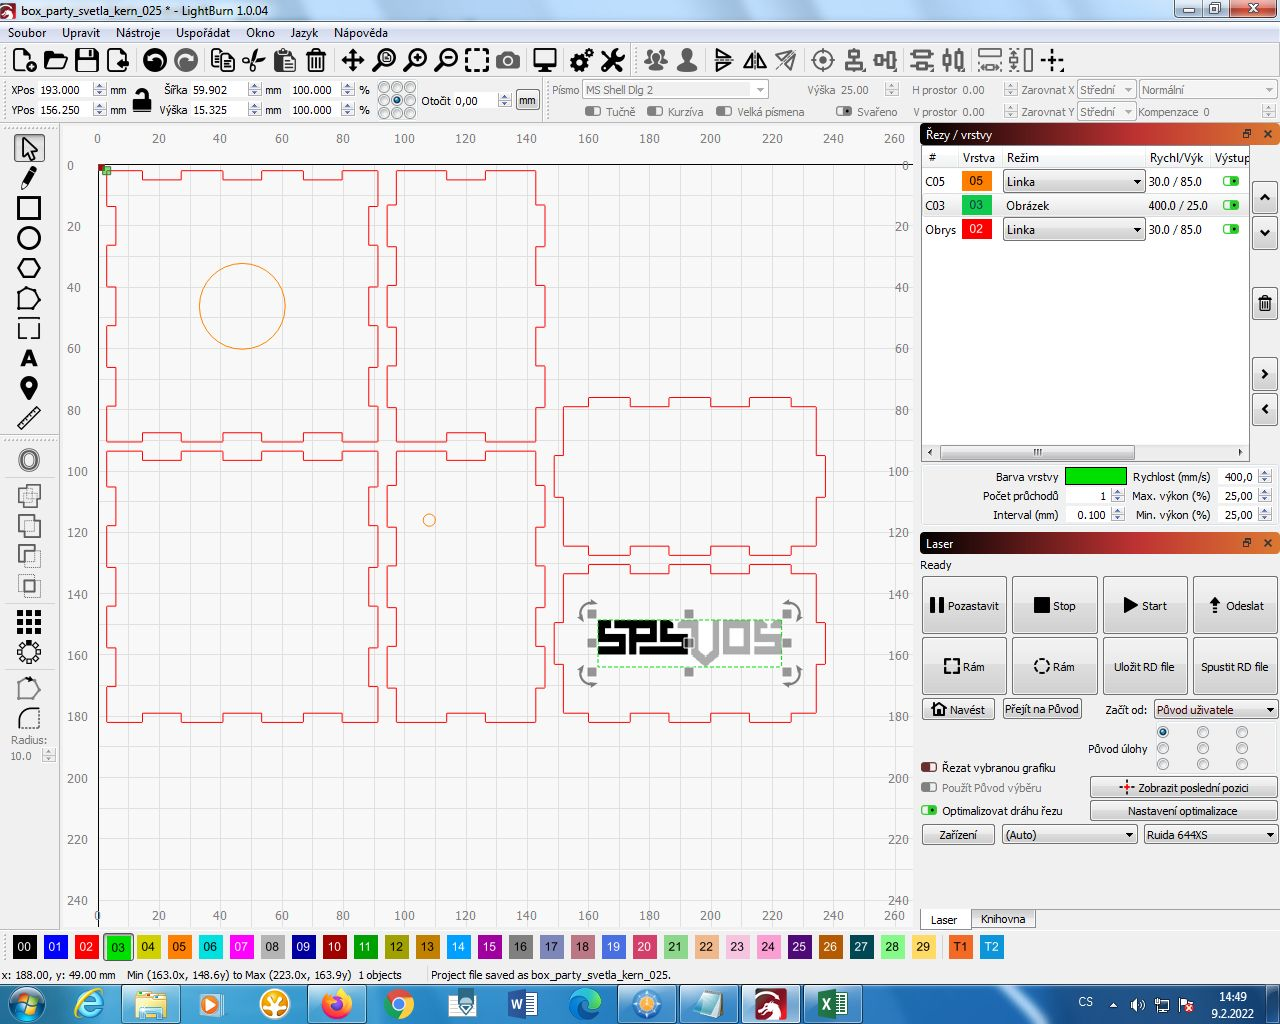
\includegraphics[width=0.5\textwidth]{img/06 zakl/LightBurn_ukazka.jpg}
	\caption{Prostředí LightBurn}
	%	\label{fig:install-sdk-3}
\end{figure}

\subsection{Vložení elektrotechniky a růže do krabičky}
Krabičky pak byly složeny do své finální podoby a jejich rohy byly zpevněny lepidlem \textit{Herkules}, aby krabičky lépe držely pohromadě. Jediný kus, který nebyl přilepen, byl vrchní díl s růží, aby se kdykoliv v případě potřeby mohl sundat. 


Poté byl vložen elektrický obvod. Přepínač byl upevněn do otvoru na tlačítko, do základny byl položen opatrně držák s bateriemi a \textit{ESP32-DevKitC} byl umístěn na kousek polystyrenu, aby v krabičce jen tak neležel a nelítal. 
%Todo lépe zdůvodnit ten polystyren, kabely byli douhé. (nevhodně ustřižené)
Ohebný LED pásek byl opatrně ohnut do obloučku a vložen do otvoru v růži. Poté bylo opatrně přiděláno vrchní víko a bylo hotovo. 
%todo nevím jak to zakončit. 

\begin{figure}[htbp]
	\centering
	\begin{minipage}[b]{0.45\textwidth}
		\centering
		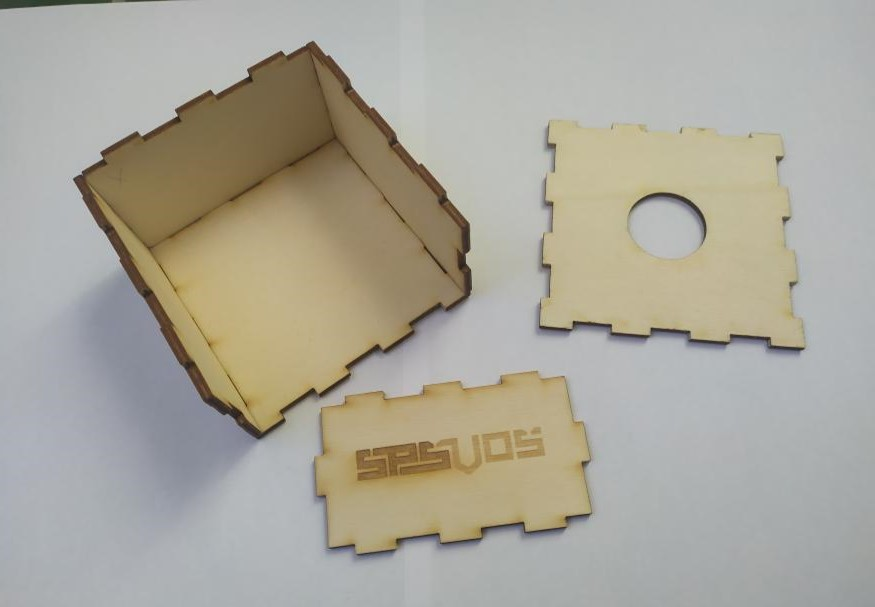
\includegraphics[width=1.1\textwidth]{img/06 zakl/Box.jpg}
		\caption{2. prototyp}
		%		\label{fig:gear-sketch1}
	\end{minipage}
	\qquad
	\begin{minipage}[b]{0.45\textwidth}
		\centering
		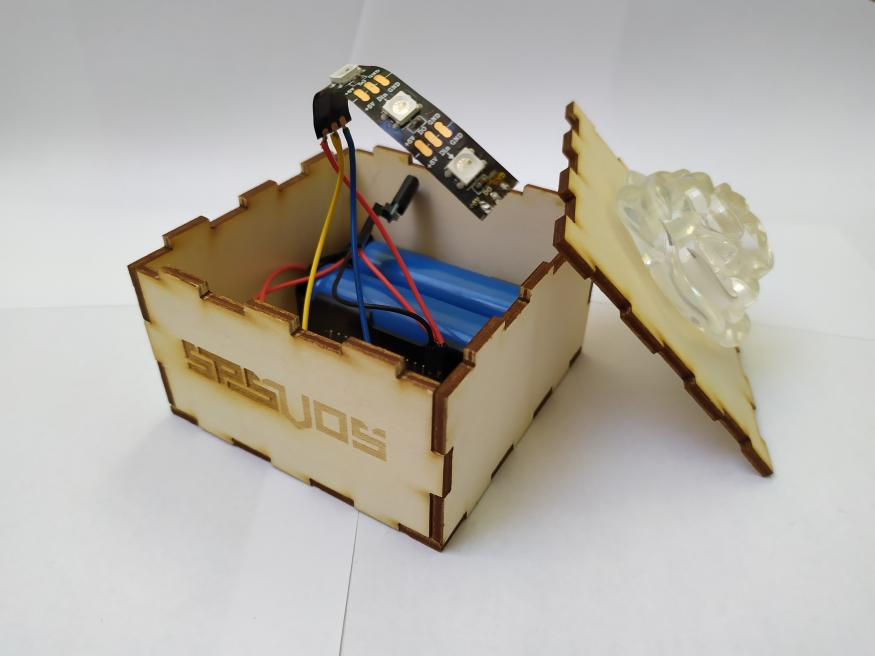
\includegraphics[width=1.01\textwidth]{img/06 zakl/2. prototyp s ele2 .jpg}
		\caption{2. prototyp s elektronikou}
		%		\label{fig:gear-sketch2}
	\end{minipage}
\end{figure}

\newpage
